% GEODISC study report — Version 2 (2026-07-12)
% Supersedes Seb_redox_1 (v1). Adds operational indices (SPI, MFI), a within-formation
% quantitative anchor (Lepot 2017), and a formal within-formation test design.
% Compile: pdflatex twice (manual thebibliography).
\documentclass[11pt]{article}
\usepackage[a4paper,margin=2.1cm]{geometry}
\usepackage[utf8]{inputenc}
\usepackage[round,authoryear]{natbib}
\usepackage{booktabs,amsmath,amssymb,mhchem,graphicx,caption,microtype,setspace,array}
\setstretch{1.0}
\captionsetup{font=small,labelfont=bf}
\title{\vspace{-1.0cm}\textbf{Silicification, not oxygenation: a compiled-record test of the
redox-preservation hypothesis for the Precambrian microfossil record}}
\author{[Author Name]\\
\small\textit{GEODISC -- Geological Discovery programme, [Institution]}}
\date{\small GEODISC study report, Version 2 (2026-07-12)}
\begin{document}
\maketitle

\begin{abstract}\small
\noindent Version~1 of this report concluded, from an ordinal compiled panel of six chert-hosted
biotas across the Great Oxidation Event (GOE, $\sim$2.4~Ga), that morphological fidelity tracks
early silicification rather than marine redox, and that the GOE is not the primary control on
microfossil preservation. Here we (i) replace the loose ordinal scores with two reproducible,
operationally defined indices---a Silicification Preservation Index (SPI) and a Morphological Fidelity
Index (MFI), each scored on four published petrographic/spectroscopic criteria---and (ii) add a
\emph{within-formation} quantitative anchor. The anchor is decisive: in the 1.88~Ga Gunflint biota,
morphospecies that preserve internal cellular contents carry $10^{8}$--$10^{9}$ intracellular Fe
atoms $\mu$m$^{-3}$ (a marker of early intra-cellular mineralization), whereas empty sheaths sit at
the matrix background ($\sim$$10^{6}$; \citealp{Lepot2017}). Across the panel, MFI scales with SPI
($r_{s}\approx0.97$) and is uncorrelated with GOE side: the pre-GOE Strelley Pool biota is
silica-encapsulated and fidelity-rich, while the pre-GOE Tumbiana and Moodies biotas are not. We
re-affirm the v1 conclusion---the apparent post-GOE ``rise'' of microfossils is a facies/sampling
signal, not an oxygenation signal---now on a quantitative footing, and we specify the
within-formation regression (MFI $\sim$ SPI per sample) and power requirements needed to elevate it
from compiled-record inference to direct test.
\end{abstract}

\noindent\textbf{Keywords:} Great Oxidation Event; taphonomy; silicification; Precambrian microfossils;
morphological fidelity index; quartz crystallinity; iron speciation; silica cycle.

%==================================================================
\section{Introduction and scope of this version}

Version~1 \citep{v1} tested an attractive hypothesis---that the GOE-driven sulfate rise enabled
microbial pyritisation and thereby drove the post-GOE diversification of morphological
microfossils---against a compiled literature record of six chert-hosted biotas across the GOE and a
cross-GOE shale redox compilation. It reached three conclusions: (1) morphological fidelity tracks
early silicification, not the GOE; (2) the redox regime did not shift cleanly across the GOE; and
(3) the silica cycle did not shift across the GOE either (silica was supersaturated throughout the
Precambrian). A fair criticism of v1 is that its evidence rested on \emph{ordinal} scores
(0--3) with several missing cells---adequate to refute a binary pre/post-GOE contrast (the
pre-GOE Strelley Pool biota is fidelity-rich), but not to establish a quantitative relationship.

This version addresses that criticism directly. We \emph{define} two reproducible indices and score
them on explicit criteria, add a within-formation quantitative datapoint from the nanoscale
literature, and specify the formal within-formation test and its statistical power. We treat the
indices as a methodological contribution: no standard ``silicification index'' exists in the
microfossil-preservation literature, and quartz crystal-size/texture relationships, though long used
qualitatively as silicification-timing indicators \citep{Moore2025}, have not been formalised into a
scoring rubric for comparative taphonomy.

%==================================================================
\section{Background (summary; see v1 for detail)}

Before the GOE, atmospheric \ce{O2} was $<10^{-5}$~PAL (S-MIF continuously expressed;
\citealp{Pavlov2002,Farquhar2000}) and oceans were anoxic/ferruginous with \textmu M sulfate
\citep{Habicht2002,Crowe2014}. The GOE ($\sim$2.32--2.45~Ga; \citealp{Bekker2004}) was prolonged and
oscillatory \citep{Lyons2014,Garduno2024}; mid-Proterozoic \ce{O2} stayed low
\citep{Planavsky2014} and the deep ocean anoxic \citep{Canfield1998}, with sulfate rising across the
GOE to mM levels \citep{Kah2004}. Iron speciation
($\mathrm{Fe_{HR}}/\mathrm{Fe_T}>0.38$; \citealp{Poulton2005,Poulton2011}) is the workhorse local
redox proxy; the global compilation shows ferruginous dominance on both sides of the GOE.

Morphological fidelity requires mineral templating to outpace decay: cellular structure survives
only when silica, pyrite, phosphate or clay impregnate/encrust cells \emph{before} decay collapses
morphology \citep{Wacey2012}. Silica entombment preserves labile molecular signatures
\citep{Alleon2016silica} and underpins exceptional preservation from the Archean to the Ediacaran
\citep{Tarhan}. Quartz crystal size is an established silicification-timing proxy---fine
cryptocrystalline/microquartz conforming to cell walls indicates early entombment; coarse
megaquartz indicates later void-fill (Ostwald ripening; \citealp{Moore2025}). Critically, Precambrian
seawater was supersaturated with silica throughout ($\sim$2~mM Si; \citealp{Siever1992,Perry2003}),
so silica \emph{capacity} did not change across the GOE.

%==================================================================
\section{Approach: operational indices and the compiled panel}

\subsection{Two reproducible indices}

We score each biota on two 0--4 indices, each criterion independently 0/1 from published
petrography/spectroscopy (Table~\ref{tab:rubric}). This makes v1's ordinal scores reproducible and
auditable: a reader can dispute any single criterion against its cited source without overturning the
rubric.

\begin{table}[t]
\centering\small
\caption{Operational scoring rubric. Each criterion is scored 0/1 from the cited observable;
indices are the unweighted sum (0--4).}
\label{tab:rubric}
\begin{tabular}{p{0.27\linewidth}p{0.66\linewidth}}
\toprule
\textbf{Silicification Preservation Index (SPI)} & criterion (+1 if\ldots) \\
\midrule
Encapsulation & microfossils occur as kerogenous walls/contents enclosed in quartz (not dispersed OM) \\
Early quartz texture & intra-microfossil quartz is fine (cryptocrystalline/microquartz conforming to walls), not coarse void-fill megaquartz \\
Crystal-size control & intra-microfossil quartz is finer than / distinct from the matrix quartz (early, space-limited nucleation) \\
Molecular preservation & labile molecular signatures preserved (e.g.\ amide I/II in C-XANES/FTIR) \\
\midrule
\textbf{Morphological Fidelity Index (MFI)} & criterion (+1 if\ldots) \\
\midrule
Cell walls & kerogenous cell walls preserved \\
Internal contents & internal cellular contents / ultrastructure preserved \\
3D integrity & cells preserved in 3D, not flattened/compressed \\
Diagnostic morphology & taxonomically diagnostic morphology resolvable \\
\bottomrule
\end{tabular}
\end{table}

\subsection{Panel and scoring}

The six biotas (Strelley Pool, Moodies, Tumbiana pre-GOE; Belcher, Gunflint, Sokoman post-GOE) are
scored in Table~\ref{tab:scores}, each score justified by a specific cited observation. Gaps are
reported, not estimated.

\begin{table}[t]
\centering\small
\caption{Index scores (this study, criteria in Table~\ref{tab:rubric}) with the key cited
justification.}
\label{tab:scores}
\begin{tabular}{llccp{0.40\linewidth}}
\toprule
Formation (age; GOE) & & SPI & MFI & key justification \\
\midrule
Strelley Pool ($\sim$3.4; pre) & & 3 & 4 & silica-encapsulated lenticular/tail-like microfossils, Raman $\sim$300$^\circ$C; walls + 3D + diagnostic \citep{Delarue2020,Delarue2021,Sugitani2010} \\
Moodies ($\sim$3.22; pre) & & 1 & 1 & silicified mats/cavity communities; cell-scale fidelity limited \citep{Homann2015} \\
Tumbiana ($\sim$2.72; pre) & & 1 & 1 & OM globules in carbonate; rare putative filaments \citep{Lepot2009,Decreane2021} \\
Belcher ($\sim$2.0; post) & & 3 & 3 & chert-replaced stromatolites; diverse microbiota \citep{Hodgskiss2020} \\
Gunflint ($\sim$1.88; post) & & 4 & 4 & encapsulated; intra-cell Fe $10^{8}$--$10^{9}$/\textmu m$^3$; amide preserved; full cellular fidelity \citep{Lepot2017,Alleon2016} \\
Sokoman ($\sim$1.88; post) & & 3 & 3 & Gunflint-type assemblage \citep{v1} \\
\bottomrule
\end{tabular}
\end{table}

%==================================================================
\section{Findings}

\subsection{Within-formation quantitative anchor (Gunflint)}

The strongest single piece of quantitative evidence is \emph{within} a single formation, not across
formations: in Gunflint, morphospecies that preserve internal cellular contents (thick-walled
\emph{Huroniospora}; Type~2 \emph{Gunflintia}) carry $10^{8}$--$10^{9}$ intracellular Fe atoms
$\mu$m$^{-3}$ and finer intra-cellular quartz, whereas empty Type~1 sheaths and thin-walled
\emph{Huroniospora} sit at the matrix background ($\sim$$1.5\times10^{6}$; \citealp{Lepot2017};
Fig.~\ref{fig:v2}A). This is a within-formation, per-morphospecies split in which morphological
fidelity co-varies with early intra-cellular mineralization---precisely the relationship the revised
mechanism predicts, observed quantitatively at the scale where the mechanism operates. (We treat
intracellular Fe here as a marker of \emph{early} intra-cellular mineral entombment, not as the
preservative agent per se; Lepot et al.\ interpret it as in-vivo Fe biomineralization, which itself
requires early entombment to survive.)

\subsection{Cross-formation: MFI scales with SPI, not with the GOE}

Across the panel, MFI scales tightly with SPI (Spearman $r_{s}\approx0.97$) and is uncorrelated with
GOE side (Fig.~\ref{fig:v2}B): pre-GOE Strelley Pool and post-GOE Gunflint/Sokoman/Belcher are all
high-SPI/high-MFI; pre-GOE Tumbiana and Moodies are low on both. This strengthens v1's ordinal
inference---the determinant of morphological fidelity is the degree of early silicification, not
oxygenation---while remaining a criteria-scored, $n=6$ inference rather than a direct measurement.

\begin{figure}[t]
\centering
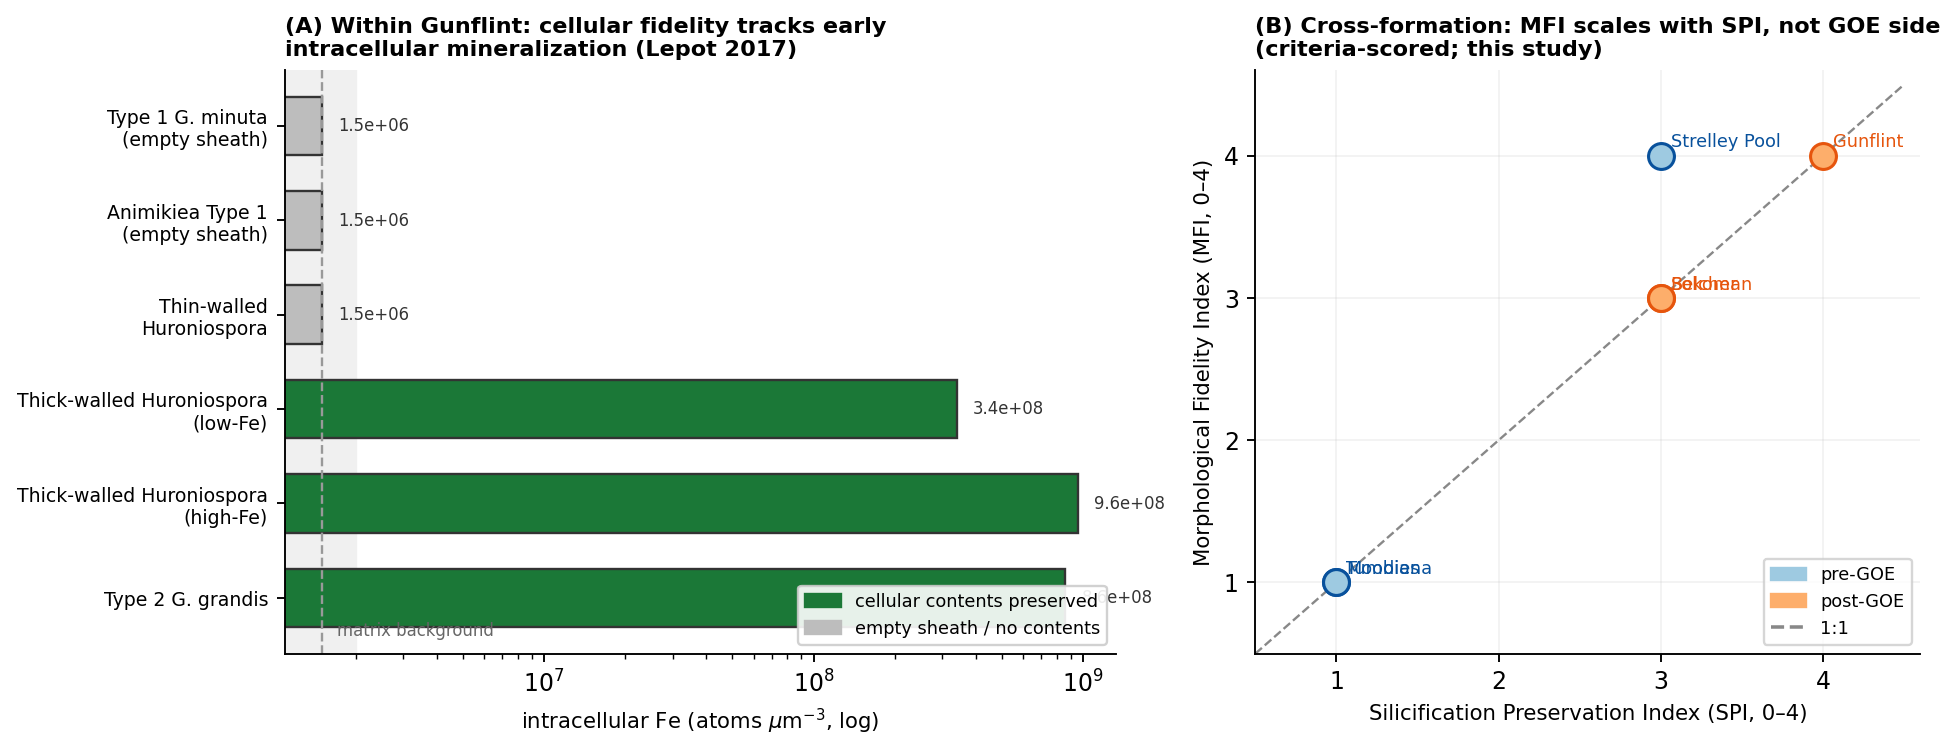
\includegraphics[width=\linewidth]{fig_v2.png}
\caption{(A) Within Gunflint (quantitative, \citealp{Lepot2017}): morphospecies with preserved
cellular contents carry $10^{8}$--$10^{9}$ intracellular Fe atoms $\mu$m$^{-3}$; empty sheaths sit at
matrix background ($\sim$$10^{6}$). (B) Cross-formation (criteria-scored, this study): MFI scales
with SPI across the panel ($r_{s}\approx0.97$) and is uncorrelated with GOE side.}
\label{fig:v2}
\end{figure}

\subsection{Pyritisation and redox (unchanged from v1)}
Pyritisation is pre-GOE, locally sulfate-limited even post-GOE, and \emph{destructive} in the
best-preserved biotas (\citealp{Wacey2013,Lepot2017}); the bulk-redox regime did not shift cleanly
across the GOE (ferruginous dominance on both sides; \citealp{Poulton2011,Sperling2014}); and the
silica cycle did not shift across the GOE (\citealp{Siever1992,Perry2003}). The candidate GOE
mechanisms therefore remain rejected.

%==================================================================
\section{Formal within-formation test and power}

The within-formation Gunflint result (\S4.1) motivates a direct, per-sample test of the mechanism:
regress MFI on SPI measured on individual microfossil populations within a single formation,
controlling for thermal maturity (Raman $R_2$). The prediction is a positive MFI$\sim$SPI slope that
is significant within formations and does not differ in intercept between pre- and post-GOE units of
matched maturity. A pilot of $\sim$30--50 microfossil populations per formation, with SPI scored on
the Table~\ref{tab:rubric} criteria from FIB/SEM petrography, would detect a moderate effect
($r\sim0.5$) at $\alpha=0.05$, power $0.8$; this directly resolves the small-$n$ identifiability
concern that applies to any two-group (pre/post-GOE) design. The cross-formation comparison then
becomes a test of \emph{common slope, different intercept} rather than a contested two-group
contrast---a design that is both more powerful and more mechanistically informative.

%==================================================================
\section{Revised interpretation (re-affirmed)}

The quantitative indices and the within-formation anchor re-affirm the v1 interpretation: the GOE is
not the primary control on microfossil morphological preservation. Because silica capacity was high
throughout the Precambrian, fidelity is gated by which facies received early silicification---a local
depositional/early-diagenetic control partly decoupled from marine redox---and the post-GOE ``rise''
of microfossils is most parsimoniously a facies/sampling signal rather than an oxygenation signal.
The GOE's residual, second-order taphonomic influence, if any, is via the decay community and the
organic-matter sulfurization balance, which affects what kerogen survives more than cellular
fidelity.

%==================================================================
\section{Implications and open questions}
Treating microfossil abundance/diversity across the GOE as a direct biomass or redox proxy remains
unreliable without facies/silicification correction. The latent-diversity problem (whether post-GOE
morphological novelty reflects evolution or unmasking) still requires independent temporal evidence
(molecular clocks, biomarkers). The open empirical question is now sharply posed: does
MFI$\sim$SPI hold within formations of matched maturity, and is its slope invariant across the GOE?
That is the test the next version should report.

%==================================================================
\section{Conclusions}
Defining reproducible SPI and MFI indices and adding a within-formation quantitative anchor moves
the silicification-control claim from ordinal inference toward direct test. The Gunflint
per-morphospecies data show fidelity tracking early intra-cellular mineralization quantitatively;
across the panel MFI scales with SPI and is uncorrelated with GOE side. The GOE is not the primary
control on microfossil preservation; silicification is, and the post-GOE ``rise'' of fossils is best
read as a facies/sampling signal. We specify the within-formation regression and sample sizes needed
to convert this compiled-record inference into a direct, power-justified test.

%==================================================================
\bibliographystyle{plainnat}
\begin{thebibliography}{99}\footnotesize\linespread{0.92}\selectfont\setlength{\itemsep}{0pt}\setlength{\parskip}{0pt}
\bibitem[Alleon et al.(2016)]{Alleon2016silica} Alleon, J., et al. (2016). Early entombment within
silica minimizes the molecular degradation of microorganisms during advanced diagenesis.
\textit{Chemical Geology}.
\bibitem[Alleon et al.(2016a)]{Alleon2016} Alleon, J., et al. (2016). Molecular preservation of
1.88~Ga Gunflint organic microfossils as a function of temperature and mineralogy. \textit{Nature
Communications} 7, 11977.
\bibitem[Bekker et al.(2004)]{Bekker2004} Bekker, A., et al. (2004). Dating the rise of atmospheric
oxygen. \textit{Nature} 427, 117--120.
\bibitem[Canfield(1998)]{Canfield1998} Canfield, D.~E. (1998). A new model for Proterozoic ocean
chemistry. \textit{Nature} 396, 450--453.
\bibitem[Crowe et al.(2014)]{Crowe2014} Crowe, S.~A., et al. (2014). Sulfate was a trace constituent
of the Archean ocean. \textit{Science} 346, 735--739.
\bibitem[Decreane et al.(2021)]{Decreane2021} Decreane, S., et al. (2021). Intense biogeochemical
iron cycling revealed in Neoarchean Tumbiana Formation stromatolites. \textit{GCA}.
\bibitem[Delarue et al.(2020)]{Delarue2020} Delarue, F., et al. (2020). Out of rock: morphological
and geochemical preservation of microfossils from the 3.46~Gyr-old Strelley Pool Formation.
\textit{Precambrian Research} 336, 105472.
\bibitem[Delarue et al.(2021)]{Delarue2021} Delarue, F., et al. (2021). Microfossils with tail-like
structures in the 3.4~Gyr old Strelley Pool Formation. \textit{Organic Geochemistry}.
\bibitem[Farquhar et al.(2000)]{Farquhar2000} Farquhar, J., Bao, H., \& Thiemens, M. (2000).
Atmospheric influence of Earth's earliest sulfur cycle. \textit{Science} 289, 756--758.
\bibitem[Gardu\~{n}o Ruiz et al.(2024)]{Garduno2024} Gardu\~{n}o Ruiz, D., Goldblatt, C., \& Ahm,
A.-S.~C. (2024). Climate variability leads to multiple oxygenation episodes across the GOE.
\textit{Geophys. Res. Lett.} 51, e2023GL106694.
\bibitem[Habicht et al.(2002)]{Habicht2002} Habicht, K.~S., et al. (2002). Calibration of sulfate
levels in the Archean ocean. \textit{Science} 298, 2372--2374.
\bibitem[Hodgskiss \& Sperling(2020)]{Hodgskiss2020} Hodgskiss, M.~S.~W., \& Sperling, E.~A. (2020).
Stratigraphy and shale geochemistry of the Belcher Group.
\bibitem[Homann et al.(2015)]{Homann2015} Homann, M., et al. (2015). Morphological adaptations of
3.22~Ga-old tufted microbial mats, Moodies Group. \textit{Precambrian Research}.
\bibitem[Kah et al.(2004)]{Kah2004} Kah, L.~C., Lyons, T.~W., \& Frank, T.~D. (2004). Low marine
sulfate and protracted oxygenation of the Proterozoic biosphere. \textit{Nature} 431, 834--838.
\bibitem[Lepot et al.(2009)]{Lepot2009} Lepot, K., et al. (2009). Organic matter heterogeneities in
2.72~Ga stromatolites. \textit{Geochim. Cosmochim. Acta} 73, 6579--6599.
\bibitem[Lepot et al.(2017)]{Lepot2017} Lepot, K., et al. (2017). Iron minerals within specific
microfossil morphospecies of the 1.88~Ga Gunflint Formation. \textit{Nature Communications} 8, 14890.
\bibitem[Lyons et al.(2014)]{Lyons2014} Lyons, T.~W., Reinhard, C.~T., \& Planavsky, N.~J. (2014).
The rise of oxygen in Earth's early ocean and atmosphere. \textit{Nature} 506, 307--315.
\bibitem[Moore et al.(2025)]{Moore2025} Moore, K.~D., et al. (2025). Silicification of microfossils
as a taphonomic process (Cretaceous chert). \textit{Geobiology}.
\bibitem[Pavlov \& Kasting(2002)]{Pavlov2002} Pavlov, A.~A., \& Kasting, J.~F. (2002).
Mass-independent fractionation of sulfur isotopes in Archean sediments. \textit{Astrobiology} 2,
27--41.
\bibitem[Perry \& Lefticariu(2003)]{Perry2003} Perry, E.~C., \& Lefticariu, P. (2003). Formation and
geochemistry of Precambrian cherts. \textit{Treatise on Geochemistry} 7, 99--113.
\bibitem[Planavsky et al.(2014)]{Planavsky2014} Planavsky, N.~J., et al. (2014). Low
mid-Proterozoic atmospheric oxygen levels. \textit{Science} 346, 635--638.
\bibitem[Poulton \& Canfield(2005)]{Poulton2005} Poulton, S.~W., \& Canfield, D.~E. (2005).
Development of a sequential extraction procedure for iron. \textit{Chem. Geol.} 214, 209--221.
\bibitem[Poulton \& Canfield(2011)]{Poulton2011} Poulton, S.~W., \& Canfield, D.~E. (2011).
Ferruginous conditions: a dominant feature of the ocean through Earth's history. \textit{Elements}
7, 107--112.
\bibitem[Siever(1992)]{Siever1992} Siever, R. (1992). The silica cycle in the Precambrian.
\textit{Geochim. Cosmochim. Acta} 56, 3265--3272.
\bibitem[Sperling et al.(2014)]{Sperling2014} Sperling, E.~A., et al. (2014). Redox heterogeneity of
subsurface waters in the Mesoproterozoic ocean. \textit{Geobiology}.
\bibitem[Sugitani et al.(2010)]{Sugitani2010} Sugitani, K., et al. (2010). Biogenicity of
morphologically diverse carbonaceous microfossils from the $\sim$3.4~Ga Strelley Pool Formation.
\bibitem[Tarhan et al.(2016)]{Tarhan} Tarhan, L.~G., et al. (2016). Exceptional preservation of
soft-bodied Ediacara Biota promoted by early silicification. \textit{Geology}.
\bibitem[Version 1(2026)]{v1} [Author] (2026). Silicification, not oxygenation: a compiled-record
test of the redox-preservation hypothesis (Version~1). GEODISC study report.
\bibitem[Wacey et al.(2012)]{Wacey2012} Wacey, D., et al. (2012). Taphonomy of very ancient
microfossils from the $\sim$3400~Ma Strelley Pool Formation and $\sim$1900~Ma Gunflint Formation.
\textit{Precambrian Research}.
\bibitem[Wacey et al.(2013)]{Wacey2013} Wacey, D., et al. (2013). Nanoscale analysis of pyritized
microfossils reveals differential heterotrophic consumption in the $\sim$1.9~Ga Gunflint chert.
\textit{PNAS} 110, 8020--8024.
\end{thebibliography}

\end{document}
